%!TEX root = ../Main.tex

\section{Evaluation}
\label{s:Evaluation}

\TODO{Discuss the performance of the system. Why this is a good idea. Give graphs that show the number of states is sensible when more processes are fused in.}


\subsection{Optimisation}
\label{s:Optimisation}
After the algorithm has completed fusing both processes it may be possible to eliminate redundant @jump@, depending on how the affected variables are used by other instructions.

\TODO{Discuss combining jump instructions here. Use this to motivate the need for drop instructions.}

\begin{figure}

\begin{minipage}[t]{0.4\textwidth}
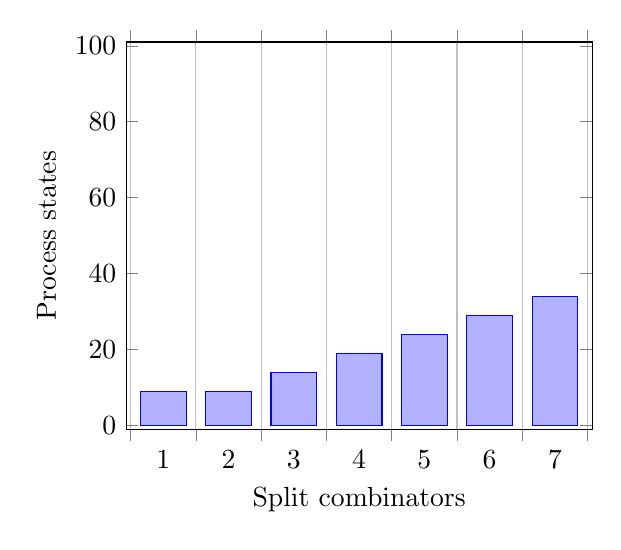
\begin{tikzpicture}
\begin{axis}[
	ylabel=Process states,
	xlabel=Split combinators,
  ymin=0, ymax=100,
	enlargelimits=0.01,
	ybar interval=0.7,
  width=7.5cm, height=6.5cm,
]
\addplot coordinates {(1,9) (2,9) (3,14) (4,19) (5,24) (6,29) (7,34)
  % Last one doesn't show for some reason, so add one above the max 
    (8,100) };
\end{axis}
\end{tikzpicture}
\end{minipage}
\begin{minipage}[t]{0.10\textwidth}
\quad
\end{minipage}
\begin{minipage}[t]{0.4\textwidth}
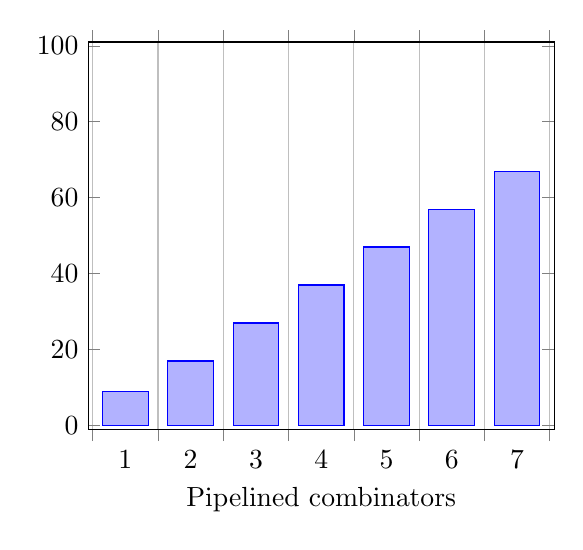
\begin{tikzpicture}
\begin{axis}[
%	ylabel=Process states,
	xlabel=Pipelined combinators,
  ymin=0, ymax=100,
	enlargelimits=0.01,
	ybar interval=0.7,
  width=7.5cm, height=6.5cm,
]
\addplot coordinates {(1,9) (2,17) (3,27) (4,37) (5,47) (6,57) (7,67)
  % Last one doesn't show for some reason, so add one above the max 
  (8,100) };
\end{axis}
\end{tikzpicture}
\end{minipage}

\caption{Maximum number of process states for all combinations of up to $n$ combinators.}
\label{fig:bench:other}
\end{figure}

